\begin{figure}[!ht]
    \centering
    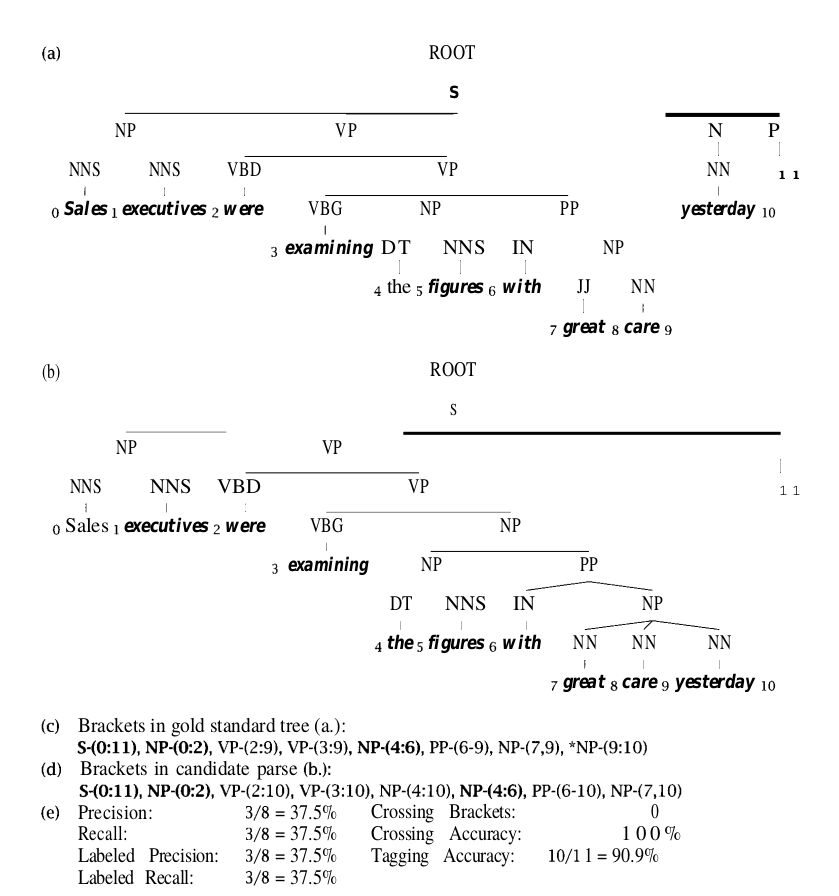
\includegraphics[width=\textwidth]{imagens/fig_demo_parseval.png}
    % \includesvg[width=.8\textwidth]{demo}
    % \includesvg{imagens/cintil_pcfg}
    \caption[Demonstração do funcionamento do PARSERVAL]{Demonstração do funcionamento do PARSERVAL. Extraido de \citeonline[p~433]{Manning1999FoundationsNLP}. Note que o nó NP-(9:10) (\textit{yesterday}), ao ser posicionado como filho do nó NP-(7:10), torna todos os nós acima dele também errados.}
    \label{fig:demo_parseval}
\end{figure}